\chapter{О влиянии пленки  поверхностно-активного вещества на дрейфовое течение, вызванное волновым возмущением поверхности вязкой жидкости} \label{ch:ch4}

\section{Введение} \label{ch:ch4/sect1}

Как было показано в предыдущих главах, распространение периодических волн по поверхности жидкости вызывает довольно сложное движение жидких частичек: петлеобразное движение в вертикальной плоскости, и медленное по сравнению с групповой и фазовой скоростью волны дрейфовое движение вдоль направления распространения волны.

До сих пор наше рассмотрение опиралось на теорию идеальной жидкости и не учитывало влияние вязкости, которая существенно усложняет явление. В работах \parencite{BelonozhkoZHTF,Belonozhko2010} в дрейфовом течении в вязкой жидкости, по которой распространяются периодические волны, были выделены две различающиеся по свойствам составляющих.

Одна компонента дрейфового течения~--- «модифицированный дрейф Стокса», имеющий ту же природу, и такой же экспоненциальный характер уменьшения скорости с глубиной, что и классический дрейф Стокса. Главное отличие модифицированного дрейфа от классического~--- экспоненциальное уменьшение скорости с течением времени (причина~--- вязкая диссипация). 

Вторая компонента~--- «добавочный дрейф»~--- движение, в которое жидкость вовлекается горизонтальными вязкими напряжениями, которые возникают благодаря тому, что горизонтальные слои жидкости, участвующие в среднем дрейфе, инициированном вышеописанным механизмом, двигаются с различными скоростями. Скорость добавочного дрейфа не экспоненциальным, а более сложным образом зависит от глубины и времени и рассчитывается с помощью специальной процедуры, предложенной в работах \parencite{BelonozhkoZHTF,Belonozhko2010}.

Целью настоящего исследования является разработка аналитической асимптотической модели, позволяющей оценивать влияние пленки поверхностно-активного вещества (ПАВ) на скорость дрейфового течения, инициируемого распространением периодических капиллярно--гравитационных волн по горизонтальной поверхности вязкой бесконечно глубокой жидкости. Также ставится задача о расчете перераспределения ПАВ вдоль поверхности жидкости, связанного с её волновым возмущением. Для правильного учета поверхностных вязких напряжений, посредством которых плёнка ПАВ взаимодействует с поверхностью жидкости, используется аналитический подход, развитый в работах \parencite{BelonozhkoZHTF,Belonozhko2010}.

  \section{Постановка задачи}
  
  Рассмотрим несжимаемую ньютоновскую жидкость с плотностью $ \rho $ и кинематической вязкостью $ \nu $, заполняющей нижнее полупространство $ z<0 $ в декартовой прямоугольной системе координат $ Oxyz $, с осью $ Oz $, направленной вертикально вверх против направления действия силы тяжести $ \mathbf{g} $. По поверхности жидкости равномерно с поверхностной плотностью $ \Gamma_{0} $ распределено ПАВ, образующее нерастворимую плёнку. Рассматривается задача определения скорости среднего дрейфового течения, возникающего в результате распространения по такой поверхности периодической капиллярно--гравитационной волны с известной длиной  $ \lambda $ и амплитудой $ \zeta $, а также изменения концентрации ПАВ, связанного с этим течением. Движение жидкости для простоты расчетов считается независящим от координаты $ y $, а направление распространения волны полагается совпадающим с направлением горизонтальной оси $ Ox $.
  
Необходимо учесть, что в процессе распространения волны на деформированной волновым движением поверхности жидкости будет происходить перераспределение ПАВ, и следовательно поверхностную плотность ПАВ следует считать функцией времени и горизонтальной координаты $ \Gamma=\Gamma \left( t, x \right) $. Локальные изменения поверхностной плотности ПАВ вызывают локальные изменения величины коэффициента поверхностного натяжения $ \gamma $. Принималось, что плёнка ПАВ и верхний слой жидкости находятся в термодинамическом равновесии, поэтому изменение локального значения поверхностной плотности ПАВ вызывает мгновенное изменение локального значения коэффициента поверхностного натяжения в соответствии с изотермой $ \gamma = \gamma \left( \Gamma \right) $, считающейся известной \parencite{Levich}, \parencite{lucassen1969eh}. 

Математическая формулировка задачи расчета возникающего в жидкости поля скоростей имеет вид \parencite{BelonozhkoPav2004}:
\begin{gather}
z<\xi: \qquad  \dfrac{\partial \mathbf{U}}{\partial t}+\left( \mathbf{U} \cdot \nabla \right) \mathbf{U}=-\dfrac{1}{\rho} \nabla p+\nu \Delta \mathbf{U}+\mathbf{g}; \qquad  \nabla \cdot \mathbf{U}=0; \qquad \label{NSPAV}
\\
z=\xi: \mspace{190mu} \dfrac{\partial \xi}{\partial t}+u \dfrac{\partial \xi}{\partial x}=v\mspace{190mu} \label{GU1PAV}
\\
p-2 \rho \nu \left( \mathbf{n} \cdot \left( \mathbf{n} \cdot \nabla \right) \mathbf{U} \right) = - \dfrac{\gamma}{\left( 1+\left( \partial_{x}\xi \right)^{2} \right)^{3/2}} \dfrac{\partial^{2} \xi}{\partial x^{2}} \label{GU2PAV}
\\
-\rho \nu \left( \left( \boldsymbol{\tau} \cdot \left( \mathbf{n} \cdot \nabla \right) \mathbf{U} \right) +\left( \mathbf{n} \cdot \left( \boldsymbol{\tau} \cdot \nabla \right) \mathbf{U} \right) \right)+\dfrac{1}{\sqrt{1+\left( \partial_{x} \xi \right)^{2}}}\dfrac{\partial \gamma}{\partial x}=0 \label{GU3PAV}
\\
\dfrac{\partial \Gamma}{\partial t}+\dfrac{1}{1+\left( \partial_{x}\xi \right)^{2}}\left( \dfrac{\partial \left( \Gamma u \right)}{\partial x}+\left( \Gamma \dfrac{\partial u}{\partial z}+ \dfrac{\partial \left( v \Gamma \right)}{\partial x} \right) \dfrac{\partial \xi}{\partial x} + \Gamma \left( \dfrac{\partial \xi}{\partial x} \right)^{2} \dfrac{\partial v}{\partial z} \right) = 0 \label{GU4PAV}
\\
z \rightarrow - \infty:\mspace{120mu} u \rightarrow 0; \mspace{120mu} v \rightarrow 0 \mspace{120mu} \label{BeskUslPAV}
\end{gather}
\begin{equation*}
\mathbf{n}=\left( -\dfrac{\partial \xi}{\partial x} \mathbf{e}_{x}+\mathbf{e}_{z}\right) \left( 1+\left( \dfrac{\partial \xi}{\partial x} \right)^{2} \right)^{-1/2}; \, \boldsymbol{\tau} = \left( \mathbf{e}_{x}+\dfrac{\partial \xi}{\partial x}\mathbf{e}_{z}\right) \left( 1+\left( \dfrac{\partial \xi}{\partial x} \right)^{2} \right)^{-1/2}
\end{equation*}
Здесь $ \mathbf{U} \equiv \mathbf{U} \left( t, x, z \right)=u\left( t, x, z \right) \mathbf{e}_{x} + v\left( t, x, z \right) \mathbf{e}_{z}$~--- эйлерово поле скоростей в жидкости, символы $ \mathbf{e}_{x, z} $ описывают орты осей $ x $ и $ z $ соответственно; давление в жидкости описывается функцией $ p \equiv p\left( t, x, z \right)  $; $ \mathbf{n} $ и $ \boldsymbol{\tau} $ определяют соответственно  внешние орты нормали и касательной к поверхности жидкости, искаженной волновым движением её поверхности  $ \xi = \xi \left( t, x \right) $. 

При решении задачи~\eqref{NSPAV}~---~\eqref{BeskUslPAV} использовался стандартный подход, при котором вместо записи начальных условий, определяющих спектр мод волнового движения в начальный момент времени, решение ищется в наиболее простом с точки зрения спектрального состава виде. Такой подход позволяет получить решение наименее громоздкое в плане аналитического описания и дальнейшего качественного анализа виде \parencite{???}.

Задача~\eqref{NSPAV}~---~\eqref{BeskUslPAV} решалась методом разложения по малому параметру, пропорциональному амплитуде волнового движения $ \varepsilon = \zeta k $. С точностью до квадратичных слагаемых искомые функции выглядят следующим образом:
\begin{equation}
\begin{matrix}
\xi=\xi_{1}+\xi_{2}+O\left( \varepsilon^{3}\right);\\
u=u_{1}+u_{2}+O\left( \varepsilon^{3}\right);\\
v=v_{1}+v_{2}+O\left( \varepsilon^{3}\right);\\
p=-\rho g z +p_{1}+p_{2}+O\left( \varepsilon^{3}\right);\\
\Gamma=\Gamma_{0}+\Gamma_{1}+\Gamma_{2}+O\left( \varepsilon^{3}\right);\\
\Gamma_{0}=const;
\end{matrix}\qquad \qquad \begin{matrix}
\xi_{j}=\xi_{j}\left( x, t \right)\\
u_{j}=u_{j}\left( x, z, t \right)\\
v_{j}=v_{j}\left( x, z, t \right)\\
p_{j}=p_{j}\left( x, z, t \right)\\
\Gamma_{j}=\Gamma_{j}\left( x, z, t \right)\\
j=1; 2.
\end{matrix}
\label{RazlozhPAV}
\end{equation}

Здесь как и ранее «$ O $» - символ порядка величины. Во всех окончательных выражениях будем раскрывать определение параметра $ \varepsilon $: $ \varepsilon = \zeta k $, $ \varepsilon^{2} = \zeta^{2} k^{2} $ и придерживаясь традиционной терминологии, применяющейся в теории волн малой, но конечной амплитуды \parencite{Nayfeh, Nayfeh1971}, называть переменные $ u_{n} $, $ v_{n} $, $ \xi_{n} $, $ p_{n} $ величинами $ n $~-го порядка малости по амплитуде волны, имея в виду что фактическим малым параметром является все же отношение амплитуды волны к её длине, которое пропорционально безразмерному параметру $ \varepsilon = \zeta k $.

Подстановка разложений~\eqref{RazlozhPAV} в соотношения~\eqref{NSPAV}~---~\eqref{BeskUslPAV} и отнесение граничных условий на невозмущенную поверхность $ z=0 $ аналогично тому, как это делалось в предыдущих пунктах и описывалось в пункте~\ref{sec:ProcSnos} приводят к выделению задач первого и второго порядков малости по амплитуде волны. 

Математическая формулировка задачи первого по амплитуде волны порядка малости имеет вид:
\begin{equation}
z<0: \qquad \qquad \dfrac{\partial \mathbf{U}_{1}}{\partial t}+\dfrac{1}{\rho} \nabla p_{1}-\nu \Delta \mathbf{U}_{1}=0; \qquad \qquad \nabla \cdot \mathbf{U}_{1}=0; \qquad \qquad \qquad \label{NSPAV1}
\end{equation}
\begin{equation}
z=0:\mspace{72mu} \dfrac{\partial \xi_{1}}{\partial t}-v_{1}=0;\qquad -\rho g \xi_{1}+p_{1}-2 \rho \nu \dfrac{\partial v_{1}}{\partial z}+\gamma_{0} \dfrac{\partial^{2}\xi_{1}}{\partial x^{2}}=0;\mspace{36mu}
 \label{GU1PAV1}
\end{equation}
\begin{equation}
-\rho \nu \left( \dfrac{\partial u_{1}}{\partial z} +\dfrac{\partial v_{1}}{\partial x} \right) +\gamma_{\Gamma} \dfrac{\partial \Gamma_{1}}{\partial x}=0; \qquad \dfrac{\partial \Gamma_{1}}{\partial t}+\Gamma_{0} \dfrac{\partial u_{1}}{\partial x}=0; \qquad
 \label{GU2PAV1}
\end{equation}
\begin{equation}
z \rightarrow - \infty:\mspace{120mu} u_{1} \rightarrow 0; \mspace{120mu} v_{1} \rightarrow 0 \mspace{108mu} \label{BeskUslPAV1}
\end{equation}

Формулировка задачи второго по амплитуде волны порядка малости состоит из выражений:
\begin{equation}
z<0: \qquad  \dfrac{\partial \mathbf{U}_{2}}{\partial t}+\dfrac{1}{\rho} \nabla p_{2}-\nu \Delta \mathbf{U}_{2}=-\left( \mathbf{U}_{1}\cdot \nabla \right) \mathbf{U}_{1}; \qquad \nabla \cdot \mathbf{U}_{2}=0; \qquad  \label{NSPAV2}
\end{equation}
\begin{equation}
z=0: \mspace{144mu} \dfrac{\partial \xi_{2}}{\partial t}-v_{2}=\xi_{1} \dfrac{\partial v_{1}}{\partial z}-u_{1} \dfrac{\partial \xi_{1}}{\partial x};\mspace{144mu}
 \label{GU1PAV2}
\end{equation}
\begin{multline}
-\rho g \xi_{2}+p_{2}-2 \rho \nu \dfrac{\partial v_{2}}{\partial z}+\gamma_{0} \dfrac{\partial^{2}\xi_{2}}{\partial x^{2}}=\\
=2 \rho \nu \xi_{1} \dfrac{\partial^{2} v_{1}}{\partial z^{2}}-\xi_{1} \dfrac{\partial p_{1}}{\partial z}-\gamma_{\Gamma} \Gamma_{1} \dfrac{\partial^{2}\xi_{1}}{\partial x^{2}}-\gamma_{\Gamma} \dfrac{\partial \xi_{1}}{\partial x} \dfrac{\partial \Gamma_{1}}{\partial x};
\label{GU2PAV2}
\end{multline}
\begin{multline}
-\rho \nu \left( \dfrac{\partial u_{2}}{\partial z} +\dfrac{\partial v_{2}}{\partial x} \right) +\gamma_{\Gamma} \dfrac{\partial \Gamma_{2}}{\partial x}= \\
=\rho \nu \left( 4 \dfrac{\partial v_{1}}{\partial z} \dfrac{\partial \xi_{1}}{\partial x}+\xi_{1} \dfrac{\partial}{\partial z} \left( \dfrac{\partial v_{1}}{\partial x} + \dfrac{\partial u_{1}}{\partial z} \right) \right) - \gamma_{\Gamma \Gamma} \Gamma_{1} \dfrac{\partial \Gamma_{1}}{\partial x}; 
 \label{GU3PAV2}
\end{multline}
\begin{equation}
 \dfrac{\partial \Gamma_{2}}{\partial t}+\Gamma_{0} \dfrac{\partial u_{2}}{\partial x}=-u_{1}\dfrac{\partial \Gamma_{1}}{\partial x}- \Gamma_{1}\dfrac{\partial u_{1}}{\partial x} - \Gamma_{0} \left( \xi_{1} \dfrac{\partial^{2} u_{1}}{\partial x \partial z}+\left( \dfrac{\partial u_{1}}{\partial z}+\dfrac{\partial v_{1}}{\partial x} \right) \dfrac{\partial \xi_{1}}{\partial x} \right); 
  \label{GU4PAV2}
\end{equation}
\begin{equation}
z \rightarrow - \infty:\mspace{120mu} u_{2} \rightarrow 0; \mspace{120mu} v_{2} \rightarrow 0 \mspace{108mu} \label{BeskUslPAV2}
\end{equation}

В список исходных данных задачи необходимо включить параметры:

\begin{equation*}
\qquad \gamma_{0} \equiv \gamma \left( \Gamma_{0} \right); \qquad \gamma_{\Gamma} \equiv \left(\dfrac{d \gamma}{d \Gamma} \right)_{0}; \qquad \gamma_{\Gamma \Gamma} \equiv \left( \dfrac{d^{2} \gamma}{d \Gamma^{2}} \right)_{0}; \qquad
\end{equation*}
Они возникают в результате разложения величины коэффициента поверхностного натяжения $ \gamma \equiv \gamma \left( \Gamma \right) $ в окрестности равновесного значения $ \gamma_{0} \equiv \gamma \left( \Gamma_{0} \right)  $. Значения $ \gamma_{\Gamma} $ и $ \gamma_{\Gamma \Gamma} $ характеризуют наклон касательной и кривизну кривой, изображающей зависимость $ \gamma = \gamma \left( \Gamma \right) $ соответственно. Для обычных ПАВ, уменьшающих поверхностное натяжение, параметр $ \gamma_{\Gamma} $ принимает отрицательные значения $ \gamma_{\Gamma}<0 $ \parencite{lucassen1969eh, Levich}.

  \section{Решение}

  Решение задачи~\eqref{NSPAV1}~---~\eqref{BeskUslPAV1} первого по амплитуде волны порядка малости хорошо известно \parencite{BelonozhkoPav2004, vakbib1} и может быть описано выражениями типа бегущей волны:
  \begin{equation}
  \begin{matrix}
  \xi_{1}=\dfrac{\zeta}{2} \exp \left( \theta \right) +C.C.;\\
  u_{1}=\dfrac{\zeta}{2}\left(A \exp \left( k z \right) +B \exp \left( q z \right) \right) \exp \left( \theta \right) +C.C.;\\
  v_{1}=\dfrac{i \zeta}{2}\left(A \exp \left( k z \right) +\dfrac{B k}{q}\exp \left( q z \right) \right) \exp \left( \theta \right) +C.C.;\\
    \Gamma_{1}=\dfrac{i \zeta}{2} k \Gamma_{0} \dfrac{A+B}{S} \exp \left( \theta \right) +C.C.;
  \end{matrix}
  \label{Resh1PAV}
  \end{equation}
  \begin{equation*}
  \qquad \qquad \theta=S t - i k x; \qquad \qquad q=\sqrt{k^{2} + \dfrac{S}{\nu}} \qquad \qquad
  \end{equation*}
или суперпозицией таких волн с различными значениями волновых чисел $ k $. Набор величин $ \left( \xi_{1}, u_{1}, v_{1}, \Gamma_{1} \right) $, определенный выражениями~\eqref{Resh1PAV}, при фиксированном значении волнового числа $ k $ образует отдельную моду волнового движения. Символ  «$ C.C. $» как и в предыдущих пунктах означает комплексно сопряженные слагаемые, а значения вспомогательных величин $ A $ и $ B $ определяются соотношениями: 
\begin{gather*}
A=i S \left( \dfrac{q}{k - q} + \dfrac{\rho \nu k S}{\rho \nu \left( k+q \right) S - k^{2} \Pi}\right); \qquad B=\dfrac{i k q S \left( 2\rho \nu S - k \Pi \right)}{\left( q-k \right) \left( \rho \nu \left( k+q \right) S - k^{2} \Pi \right)};
\\
\Pi = \gamma_{\Gamma} \Gamma_{0}.
\end{gather*}
Параметр $ \Pi $ называют упругостью пленки. Он имеет размерность силы на единицу длины и характеризует упругие свойства пленки ПАВ \parencite{??} и также как $ \gamma_{\Gamma} $ для обычных ПАВ, принимает отрицательные значения \parencite{lucassen1969eh}, \parencite{??}. Изменение модуля $ \Pi $ для определенного ПАВ можно осуществить изменяя среднее значение концентрации $ \Gamma_{0} $: при нулевой средней концентрации $ \Pi=0 $ и $ \vert \Pi \vert $ растет с ростом средней концентрации $ \Gamma_{0} $. 

Комплексная частота $ S $ связана с волновым числом и другими параметрами задачи дисперсионным соотношением \parencite{BelonozhkoGrig2004}:

\begin{equation}
\left( \left( \Omega +2N \right)^{2} +1-\dfrac{L}{\Omega^{2}} \right) \left( 1-L \dfrac{1+\Omega^{2}}{4 \Omega^{2} N^{2}}\right)^{-1}=4N^{3/2} \sqrt{\Omega +N};
\label{DispUrPAV}
\end{equation}
\begin{equation*}
\Omega \equiv \dfrac{S}{\omega_{0}}; \qquad N \equiv \dfrac{\nu k^{2}}{\omega_{0}}; \qquad L \equiv \dfrac{\Pi k^{3}}{\rho \omega_{0}^{2}}; \qquad \omega_{0}^{2}=k g \left( 1+\dfrac{\gamma_{0}}{\rho g}k^{2}\right).
\end{equation*}

В дальнейшем для действительной и мнимой части комплексной частоты  используются обозначения:
\begin{equation*}
r=Re\left( S \right); \qquad \qquad \qquad \qquad \omega=Im\left( S \right).
\end{equation*}

Использованный здесь вспомогательный параметр $ \omega_{0} $ имеет смысл круговой частоты волнового движения на поверхности бесконечно глубокой идеальной жидкости с капиллярной постоянной, равной $ \sqrt{\gamma_{0}/\left( \rho g \right)} $. Безразмерный параметр $ N $ характеризует роль вязкости при волновом движении. Если $ N\ll 1 $, то жидкость принято считать маловязкой \parencite{???}.
  
  

Анализ дисперсионного уравнения показывает, что в отсутствии пленки ПАВ уравнение~\eqref{DispUrPAV} сводится к известному дисперсионному уравнению для капиллярно--гравитационных волн на поверхности бесконечно глубокой вязкой жидкости \parencite{Levich}:
\begin{equation}
\left( S+2 \nu k^{2} \right)^{2} + \omega_{0}^{2} = 4 \nu^{2} k^{3} \sqrt{k^{2}+\dfrac{S}{\nu}}
\label{DispurVyaz}
\end{equation}

Уравнение~\eqref{DispurVyaz} имеет четыре корня, однако, физический смысл имеют не все значения комплексной частоты $ S $, разрешающие дисперсионное уравнение, а только те, для которых выполняется соотношение:
\begin{equation*}
Re \left( \left( S+2 \nu k^{2} \right)^{2} + \omega_{0}^{2} \right)>0
\end{equation*}
Это условие обеспечивает положительность действительной части величины $ q $, отвечающей за затухание с глубиной (при $ z \rightarrow - \infty $) вихревой части поля скоростей~--- слагаемых, которые пропорциональны $ \propto \exp \left( q z \right) $. Другая пара корней оказывается физически нереализуемой. Физически реализуемые корни являются комплексно сопряженными и определяют две простейшие синусоидальные капиллярно--гравитационные волны, бегущие в противоположных направлениях: вдоль положительного направления оси $ Ox $ и против него. 

С учетом слагаемых, отвечающих за присутствие пленки ПАВ на поверхности жидкости дисперсионное уравнение~\eqref{DispUrPAV} имеет уже восемь корней, однако физический смысл имеют корни, удовлетворяющие соотношению:
\begin{equation*}
Re \left( \left( \left( \Omega + 2 N^{2} \right)^{2} + 1 - \dfrac{L}{\Omega^{2}}\right) \left( 1- L \dfrac{1+\Omega^{2}}{4 \Omega^{2}N^{4}}\right)^{-1}\right) >0,
\end{equation*}
обеспечивающему положительность действительной части величины $ q $. Таких корня оказывается четыре. Два из них при отсутствии ПАВ ($ \Pi \rightarrow 0 $) переходят в пару физически реализуемых корней уравнения~\eqref{DispurVyaz}. И отвечают за распространение капиллярно--гравитационных волн. Вторая пара корней принимает ненулевые значения только в присутствии пленки ПАВ ($ \Pi \neq 0 $). Эти корни определяют частоты волновых движений Марангони \parencite{BelonozhkoGrig2004}, инициируемых касательными натяжениями, возникающими в упругой пленке при распространении волн сжатий и растяжений. Стоит отметить, что капиллярно--гравитационные волны при распространении также вызывают волны сжатий и растяжений в упругой пленке, но такой волновой режим не принято считать волнами Марангони.


\section{Перераспределение ПАВ, связанное с волновым возмущением поверхности жидкости}


Изобразим зависимости частоты волнового движения $ \omega $ от модуля упругости пленки ПАВ $ \vert \Pi \vert $, полученные при решении уравнения~\eqref{DispUrPAV} для обоих типов волнового движения для различных волновых чисел. Здесь и далее в этой главе расчеты и построения выполнены в безразмерных переменных, в которых $ \rho = g = \gamma_{0}=1 $ при значении безразмерной вязкости $ \nu = 0.002 $, что соответствует вязкости воды при нормальных условиях. Линии, соответствующие капиллярно--гравитационному волновому движению помечены символом <<$ C-G $>>, а линии, соответствующие волнам Марангони~--- символом <<$ M $>>. Анализ решения показывает, что частота капиллярно--гравитационных волн практически не зависит от модуля упругости пленки ПАВ, а частота волн Марангони быстро возрастает с увеличением $ \vert \Pi \vert $. 
\begin{figure}[ht]
\centering
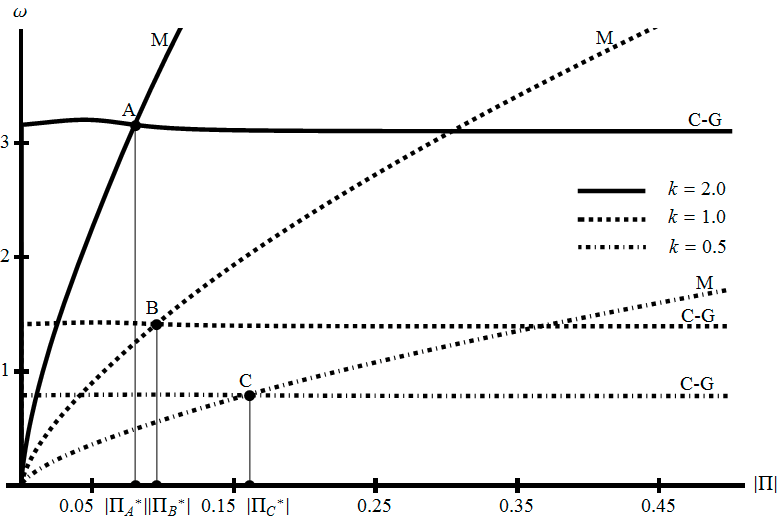
\includegraphics[scale=0.6]{fig1Pav}
\caption{Зависимость циклической частоты волнового движения Марангони и капиллярно--гравитационного волнового движения от модуля упругости пленки ПАВ для разных длин волн.}\label{fig:Fig1PAV}
\end{figure} 
Из рисунка~\ref{fig:Fig1PAV} видно, что при некотором значении модуля упругости пленки $ \vert \Pi \vert = \vert \Pi* \vert \left( k \right) $ частоты волн Марангони  сравниваются с частотой капиллярно--гравитационного волнового движения. Примечательно, что при значении модуля упругости можно заметить еще одну особенность волнового движения. Она хорошо иллюстрируется на рисунке~\ref{fig:Fig2PAV}, на котором построены зависимости декремента затухания капиллярно--гравитационных волн от модуля упругости пленки ПАВ.
\begin{figure}[ht]
\centering
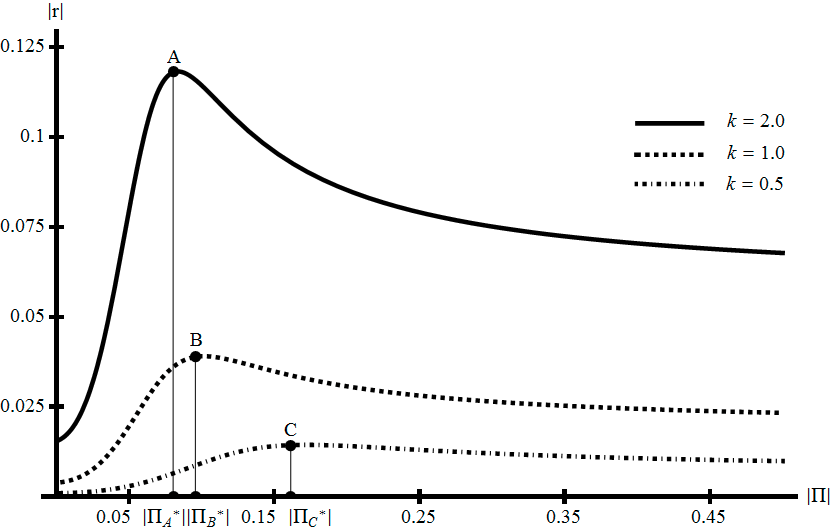
\includegraphics[scale=0.55]{fig2Pav}
\caption{Зависимость декремента затухания капиллярно--гравитационного волнового движения от модуля упругости пленки ПАВ для разных длин волн.}\label{fig:Fig2PAV}
\end{figure} 
На рисунке~\ref{fig:Fig2PAV} не изображены декременты затухания волн Марангони, так как эти зависимости очень быстро растут с увеличением упругости пленки и в масштабе рисунка~\ref{fig:Fig2PAV} сливаются с вертикальной осью. Из рисунка~\ref{fig:Fig2PAV} видно, что при достижении упругостью пленки характерного значения $ \vert \Pi \vert = \vert \Pi* \vert \left( k \right) $  декремент затухания капиллярно--гравитационных волн достигает максимума $ \vert r \vert = \vert r* \vert $, что соответствует наиболее эффективному гашению волн пленкой ПАВ. Дальнейшее увеличение упругости приводит к уменьшению декремента затухания и при $ \vert \Pi \vert \rightarrow \infty $ модуль декремента затухания стремится к своему асимптотическому значению, составляющему примерно половину от максимального $ \vert r \vert \rightarrow \vert r_{ass} \vert \approx 0.5 \vert r* \vert  $. На практике оказывается, что при ненулевых значениях модуля упругости пленки ПАВ декременты затухания волн Марангони во много раз превосходят декременты капиллярно--гравитационных волн. В связи с этим на практике наблюдение волнового движения Марангони затруднено и возможно только при постоянном притоке энергии. 
\textit{
\textbf{Максимум затухания можно объяснить тем, что происходит обмен энергией между волнами разного типа, имеющих одинаковую частоту. И из-за сильного затухания волн Марангони энергия волнового движения рассеивается и, как следствие, капиллярно--гравитационные волны тоже затухают быстрее.}} Этот эффект заметно проявляется в области капиллярных волн и несущественен в области гравитационного волнового движения (с волновым числом $ k<1 $). Ранее и экспериментально и теоретически исследовалось затухание капиллярно--гравитационных волн, связанное с присутствием ПАВ на поверхности жидкости, но оставалась без внимания интересная взаимосвязь между положением максимального декремента  распределения поверхностной концентрации ПАВ.

Интересно понаблюдать за соотношением между фазами волнового возмущения поверхности жидкости и положения максимального значения концентрации ПАВ. На рисунке~\ref{fig:Fig3PAV} изображены зависимости 	разности фаз $ \Phi $ между капиллярно--гравитационной волной, возмущающей поверхность жидкости и связанной с ней волной перераспределения концентрации ПАВ~\eqref{Resh1PAV} от модуля упругости пленки ПАВ $ \vert \Pi \vert $ для разных волновых чисел. 
\begin{figure}[ht]
\centering
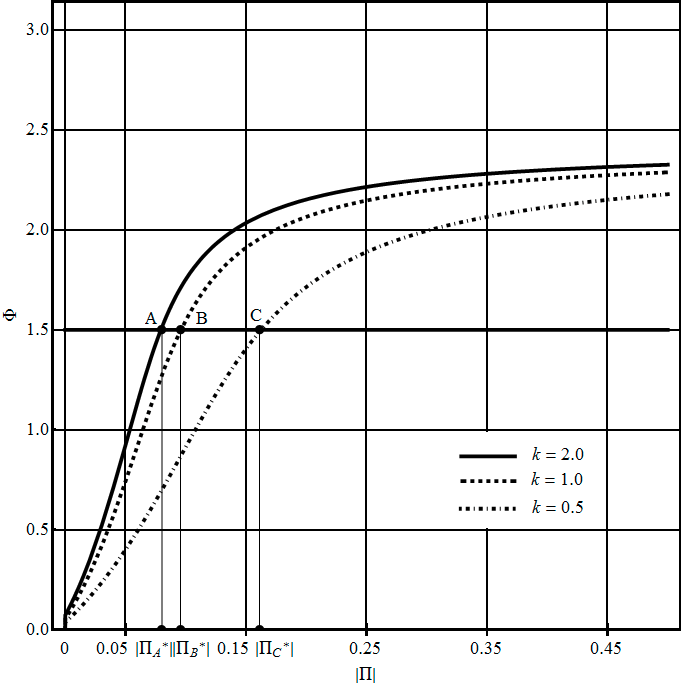
\includegraphics[scale=0.6]{fig3Pav}
\caption{Зависимость разности фаз между положением максимума концентрации ПАВ и гребнем волны для капиллярно--гравитационного волнового движения от модуля упругости пленки ПАВ.}\label{fig:Fig3PAV}
\end{figure} 	
Из рисунка~\ref{fig:Fig3PAV} видно, что при достижении максимального эффекта гашения волн (достижения модулем упругости пленки ПАВ соответствующего значения $ \vert \Pi* \vert $) разность фаз $ \Phi $ для всех длин волн оказывается примерно равной $ \pi/2 $. Это соответствует положению максимума концентрации ПАВ на середине склона волны, следующего за горбом. С уменьшением упругости пленки разность фаз уменьшается и максимум оказывается ближе к вершине горба волнового возмущения поверхности жидкости. Увеличение упругости приводит к росту разности фаз и соответственно смещению максимума концентрации ближе ко впадине волнового возмущения.
	
\section{Траектории движения индивидуальных жидких частиц в линейном приближении}
Из решения задачи первого порядка малости по амплитуде волны~\eqref{Resh1PAV} можно оценить влияние поверхностно-активного вещества на траектории движения индивидуальных частиц жидкости. Как было показано ранее в линейном приближении можно перейти от поля скоростей в описании Эйлера к полю скоростей в описании Лагранжа при помощи формальной замены пространственных эйлеровых координат на лагранжевы: $ x \rightarrow x_{0} $ и $ z \rightarrow z_{0} $. Тогда поле скоростей в описании Лагранжа можно записать в виде:
\begin{gather}
 \begin{matrix}
u_{L1}=\dfrac{\zeta}{2}\left(A \exp \left( k z_{0} \right) +B \exp \left( q z_{0} \right) \right) \exp \left( S t - i k x_{0} \right) +C.C.;\\
v_{L1}=\dfrac{i \zeta}{2}\left(A \exp \left( k z_{0} \right) +\dfrac{B k}{q}\exp \left( q z_{0} \right) \right) \exp \left( S t - i k x_{0} \right) +C.C.
  \end{matrix}
 \label{Ulagr1Pav}
\end{gather}

Прямое интегрирование выражений~\eqref{Ulagr1Pav} по времени позволяет получить параметрическое описание траектории движения индивидуальной частицы жидкости в первом приближении по амплитуде волны. 

Рассмотрим в качестве примера траектории движения индивидуальной жидкой частицы, находящейся в начальный момент времени на середине переднего склона волны с безразмерным волновым числом $ k=1 $. На рисунке~\ref{fig:PavTraj1} изображены траектории движения индивидуальной жидкой частицы при различных значениях упругости пленки ПАВ с указанием направления движения. Для того, чтобы оценить влияние ПАВ на траектории достаточно построить путь, описываемый частицей за время одного периода волнового движения. Видно, что при отсутствии ПАВ частицы совершают движение по окружностям уменьшающегося за счет вязкости радиуса (сплошная линия на рисунке). С увеличением модуля упругости пленки траектории <<сплющиваются>> в эллипсы (длинная пунктирная и штрихпунктирная линия  на рисунке) и при достижении упругостью характерного для этой длины волны значения $ \vert \Pi_{B}^{*} \vert $ вырождаются в отрезки прямых (штриховая линия на рисунке), наклоненных к горизонтальной оси под углом примерно $ \pi/4 $. 

\begin{figure}[ht]
\centering
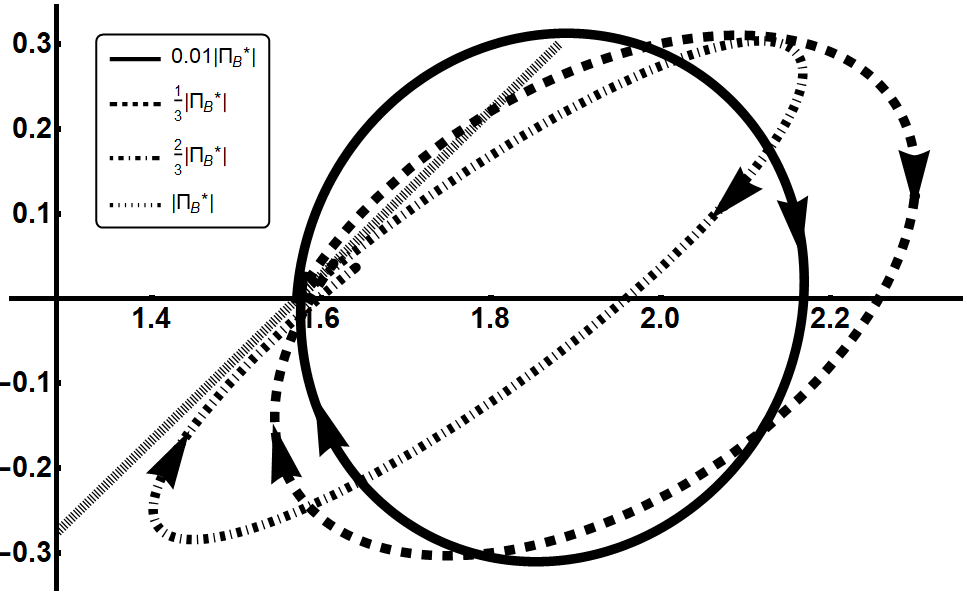
\includegraphics[scale=0.5]{fig4PavTraj1}
\caption{Траектории движения индивидуальной жидкой частицы в присутствии ПАВ с упругостью  меньше характерного значения $ \vert \Pi* \vert $ }\label{fig:PavTraj1}
\end{figure} 

Дальнейшеё увеличение упругости пленки ПАВ приводит к тому, что траектории снова <<разворачиваются>> в эллипсы (см. рисунок~\ref{fig:PavTraj2}). При этом направление движения жидких частиц сменяется на противоположное. Можно заметить, что при устремлении упругости к бесконечности траектории также вырождаются в отрезки прямых, но при этом движение жидкие частицы совершают вдоль вертикальной оси.

\begin{figure}[ht]
\centering
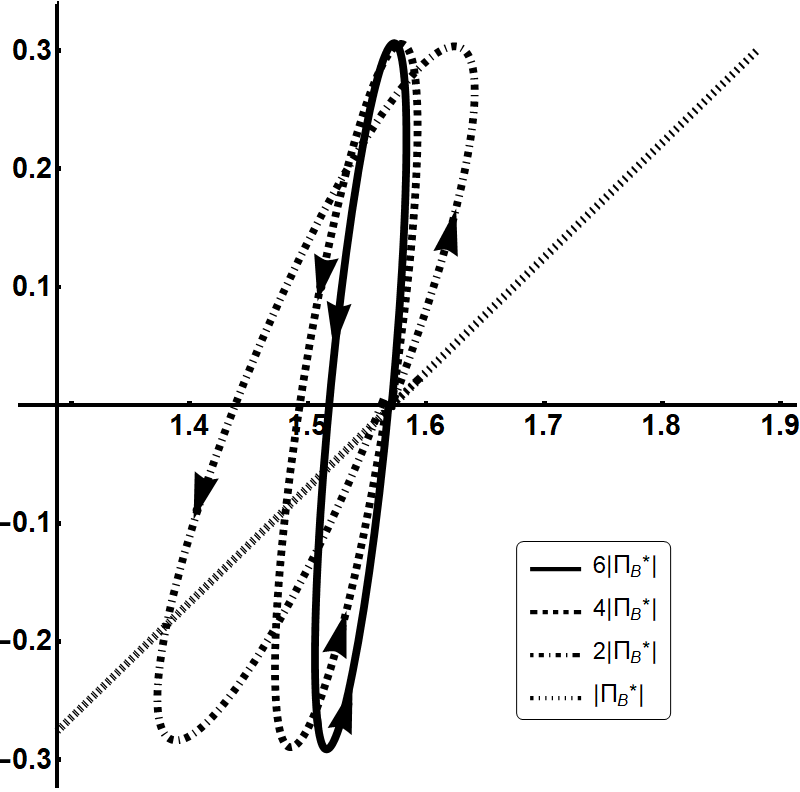
\includegraphics[scale=0.6]{fig5PavTraj2}
\caption{Траектории движения индивидуальной жидкой частицы в присутствии ПАВ с упругостью  больше характерного значения $ \vert \Pi* \vert $ }\label{fig:PavTraj2}
\end{figure} 

Такое влияние ПАВ на траектории можно объяснить следующим образом: в отсутствии пленки ПАВ на поверхности на жидкую частицу действуют капиллярно~--гравитационные силы, заставляющие её совершать вращательные движения по часовой стрелке (если волна распространяется вправо). С появлением ПАВ возникают тангенциальные упругие силы Марангони, которые направлены таким образом, что момент этих сил направлен в противоположную сторону. Это искажает круговые траектории. При достижении характерного значения $ \vert \Pi* \vert $ эти силы сравниваются и прекращается круговое движение. С превышением характерного значения упругие силы Марангони начинают преобладать, поэтому наблюдается вращение в противоположную сторону. 

\section{Дрейфовые компоненты поля скоростей}	

Решение задачи второго по амплитуде волны порядка малости, в отличие от задачи первого порядка малости, имеет составляющую, описывающую явный дрейф жидкости вдоль оси $ Ox $.В рамках концепции поиска решений с точностью до лидирующих слагаемых для каждого типа движения ограничимся установлением вида именно этой части решения.  Примем, что решение исходной задачи~\eqref{NSPAV}~---~\eqref{BeskUslPAV} в первом по амплитуде волны приближении описывается только одной модой волнового движения~--- набором соотношений вида~\eqref{Resh1PAV} с заданным значением волнового числа $ k $. 

Подставляя~\eqref{Resh1PAV} в правую часть~\eqref{NSPAV2}~---~\eqref{GU4PAV2} даже без подробных расчетов несложно установить характер их строения. Правая часть каждого соотношения представляет собой сумму двух различных по характеру слагаемых. Одно слагаемое не зависит от горизонтальной координаты $ x $ и пропорционально $ \propto \exp \left( 2 r t \right) $, а второе является суммой компонент, пропорциональных выражениям:
\begin{equation*}
\propto \exp \left( 2 r t \right) \cos \left( \omega t - k x \right); \qquad \qquad \propto \exp \left( 2 r t \right) \sin \left( \omega t - k x \right).
\end{equation*}
Слагаемые первого типа далее будем называть <<нециклические>> или <<непериодические>>, а второго~--- «циклические», поскольку их величины при фиксированных координатах циклически изменяются со временем около нулевого среднего значения. 

	Характер строения правых частей соотношений~\eqref{NSPAV2}~---~\eqref{GU4PAV2} позволяет заключить, что неизвестные $ u_{2} $, $ v_{2} $, $ p_{2} $ следует искать в виде выражений следующего общего строения:
	\begin{equation}
	u_{2}=u_{a}+\Theta; \qquad \qquad v_{2}=\Theta; \qquad \qquad p_{2}=p_{a}+\Theta;
\label{Resh2PAVVid}	
	\end{equation}
	\begin{equation*}
	u_{a} \equiv u_{a} \left( t, z \right); \qquad \qquad p_{a} \equiv p_{a} \left( t, z \right).
	\end{equation*}
Здесь символ $ \Theta $ использован для общего обозначения слагаемых циклического типа вне зависимости от их конкретного вида. Вертикальная компонента скорости $ v_{2} $ имеет только циклическую составляющую из-за того, что должен отсутствать поток жидкости в вертикальном направлении.

В результате подстановки выражений общего строения для величин второго порядка малости по амплитуде волны~\eqref{Resh2PAVVid} в соотношение, представляющее собой проекцию уравнения~\eqref{NSPAV2} на ось $ Ox $; в граничное условие~\eqref{GU3PAV2} и в условие~\eqref{GU4PAV2}, выделяется самостоятельная задача для определения $ u_{a} $:
\begin{equation}
z<0:\mspace{108mu} \dfrac{\partial u_{a}}{\partial t}- \nu \dfrac{\partial^{2} u_{a}}{\partial z^{2}}=\zeta^{2}F\left( z \right) \exp \left( 2 r t \right) \mspace{108mu}
\label{UaPAV1}
\end{equation}
\begin{equation}
z=0:\mspace{130mu} \dfrac{\partial u_{a}}{\partial t}- \nu \dfrac{\partial u_{a}}{\partial z}=\zeta^{2}G \exp \left( 2 r t \right) \mspace{130mu}
\label{UaPAV2}
\end{equation}
\begin{multline*}
F\left( z \right) \equiv i k \dfrac{\vert B \vert^{2} \left( q^{2}-q^{*2}\right)}{4 \vert q \vert^{2} \left( 2 r-\nu \left( q + q^{*} \right)^{2}\right)} \exp \left( \left( q+q^{*}\right) z \right)+ \\
+\left( \dfrac{i A^{*} B \left( q^{2} - k^{2} \right)}{4 q \left( 2 r - \nu \left( q+k \right)^{2} \right)} \exp \left( \left( q+k\right) z \right) +C.C. \right)
\end{multline*}
\begin{equation*}
G \equiv \dfrac{1}{4}\left( k^{2} \left( 2 A + 3 B \right) - B q^{2} + C.C. \right).
\end{equation*}

По явному виду правой части~\eqref{UaPAV1}~---~\eqref{UaPAV2} методом неопределенных коэффициентов несложно найти подстановку:
\begin{equation}
u_{a}=u_{b}+u_{c}
\label{Ub+Uc}
\end{equation}
\begin{multline}
u_{b} \equiv u_{b} \left( z, t \right) = \zeta^{2}  i k \dfrac{\vert B \vert^{2} \left( q^{2}-q^{*2}\right)}{4 \vert q \vert^{2} \left( 2 r-\nu \left( q + q^{*} \right)^{2}\right)} \exp \left( 2 r t+ \left( q+q^{*}\right) z \right)+ \\
+\zeta^{2} \left( \dfrac{i A^{*} B \left( q^{2} - k^{2} \right)}{4 q \left( 2 r - \nu \left( q+k \right)^{2} \right)} \exp \left( 2 r t +\left( q+k\right) z \right) +C.C. \right),
\label{Ub}
\end{multline}
редуцирующую задачу~\eqref{UaPAV1}~---~\eqref{UaPAV2} в задачу с однородным уравнением:
\begin{equation}
z<0: \qquad  \dfrac{\partial u_{c}}{\partial t}- \nu \dfrac{\partial^{2} u_{c}}{\partial z^{2}}=0; \qquad \qquad z=0:\qquad  \dfrac{\partial u_{c}}{\partial z}=\zeta^{2} \Lambda \exp \left( 2 r t \right).
\label{UcPAV}
\end{equation}
\begin{multline*}
\Lambda \equiv - i k \dfrac{\vert B \vert^{2} \left( q^{2}- q^{*2} \right) \left( q+q^{*} \right)}{4 \vert q \vert^{2} \left( 2 r - \nu \left( q+q^{*}\right)^{2} \right) }+ \\
+\left(\dfrac{1}{4} \left( k^{2} \left( 2 A+ 3 B \right) - q^{2} B \right) - i \dfrac{A^{*} B \left( q^{2} - k \right) \left( q+k \right) }{q \left( 2 r - \nu \left( q+k \right)^{2} \right)}+C.C. \right)
\end{multline*}

Таким образом, нециклическая часть решения задачи второго порядка малости  (см.~\eqref{Ub+Uc}) состоит из компоненты $ u_{b}\equiv u_{b}\left( t, z \right) $, определенной выражением~\eqref{Ub}, и компоненты $ u_{c}\equiv u_{c}\left( t, z \right) $, являющейся решением задачи~\eqref{UcPAV}. Решение будет однозначным, если задачу~\eqref{UcPAV} дополнить начальным условием, задающим вид функции $ u_{c}\left( t, z \right) $ в начальный момент времени.

Для определения средней скорости дрейфового движения воспользуемся формулой~\eqref{Pereh} и методикой пересчета известного эйлерова поля скоростей в лагранжево. описанной в пункте~\ref{sec:Pereh}. Окончательное выражение для скорости дрейфа складывается из нециклических слагаемых $ w_{d} $, полученных при вычислении интегралов в~\eqref{Pereh}, а также из  $ u_{b} $ и  $ u_{c} $:
\begin{equation}
U_{drift}=w_{d}+u_{b}+u_{c};
\label{UdriftPAV}
\end{equation}
\begin{multline}
w_{d}= \zeta^{2} \dfrac{\exp \left( 2 r t \right)}{2 \vert S \vert^{2}}\left( 2 \vert A \vert^{2} k \omega \exp \left( 2 k z \right)+ M_{0} \exp \left( 2 \beta z \right) +\right.\\
\left.+\left( M_{1}\cos \left( \eta z \right) +M_{2} \sin \left( \eta z \right) \right) \exp \left( \left( k+\beta \right) z \right) \right)
\label{wdPAV}
\end{multline}
\begin{gather*}
M_{0}= k \vert B \vert^{2} Im \left( \left( \dfrac{q}{q^{*}}+1 \right) S \right);\\
M_{1}=Im \left( A^{*} B \left( q S - \dfrac{k^{2}}{q}S^{*} \right) \right)+2 Re \left( A B^{*} \right) k Im \left( S \right);\\
M_{2}=Re\left( A^{*} B \left( q S - \dfrac{k^{2}}{q}S^{*} \right) \right) + 2 Im \left( A B^{*} \right) k Im \left( S \right).
\end{gather*}

Компонента $ u_{b} $ вычисляется по  формуле~\eqref{Ub}, а слагаемое $ u_{c} $, являясь решением задачи~\eqref{UcPAV} определяется формулой:
\begin{multline}
u_{c} \equiv u_{c} \left( z, t \right) = \zeta^{2} \Lambda \left( \sqrt{\dfrac{\nu}{\pi}} \int_{0}^{t} \exp \left( - \dfrac{z^{2}}{4 \nu \left( t - \eta \right)} \right) \dfrac{\exp \left( 2 r \eta \right)}{\sqrt{t - \eta}}d \eta +\right.\\
\left. + \sqrt{\dfrac{1}{\pi \nu t}} \int_{0}^{\infty} \left( \exp \left( -\dfrac{\left( z - \sigma \right)^{2}}{4 \nu t} \right) + \exp \left( -\dfrac{\left( z + \sigma \right)^{2}}{4 \nu t} \right) \right) \Psi \left( \sigma \right) d \sigma\right);
\label{UcYavVid}
\end{multline}
\begin{equation*}
\Psi \left( z \right) \equiv u_{c}\left( 0, z \right)
\end{equation*}

В пределе, когда отсутствует плёнка ПАВ ($ \Pi=0 $) с помощью известных асимптотических соотношений \parencite{BelonozhkoKozin2009}
\begin{gather*}
\dfrac{r}{\omega_{0}}=-2 N + O \left( N^{3/2} \right); \qquad \qquad \dfrac{\omega}{\omega_{0}}=1+O \left( N^{3/2} \right);\\
\dfrac{q}{k}=\dfrac{1+i}{\sqrt{2 N}}-\dfrac{1-i}{2 \sqrt{2}}\sqrt{N}-i N +O \left( N^{3/2} \right)
\end{gather*}
несложно найти приближенные выражения для первых двух слагаемых $ w_{d} $ и $ u_{b} $ суммы~\eqref{UdriftPAV}, справедливые в приближении малой вязкости ($ N\ll 1 $):
\begin{equation*}
w_{d}\approx \zeta^{2} k \omega_{0} \exp \left( - 4 \nu k^{2} t \right) - \zeta^{2} k \omega_{0} \cos \left( z \sqrt{\dfrac{\omega_{0}}{2 \nu}} \right) \exp \left( \left( k+ \sqrt{\dfrac{\omega_{0}}{2 \nu}} \right) z \right) \exp \left( - 4 \nu k^{2} t \right);
\end{equation*}
\begin{equation*}
u_{b}\approx \zeta^{2} k \omega_{0} \cos \left( z \sqrt{\dfrac{\omega_{0}}{2 \nu}} \right) \exp \left( \left( k+ \sqrt{\dfrac{\omega_{0}}{2 \nu}}\right) z \right) \exp \left( - 4 \nu k^{2} t \right).
\end{equation*}
Из этих приближенных равенств следует, что при малой вязкости:
\begin{equation*}
w_{d}+u_{b} \approx \zeta^{2} k \omega_{0} \exp \left( k z \right) \exp \left( - 4 \nu k^{2} t \right).
\end{equation*}

Получившееся справа выражение с точностью до множителя $ \exp \left( - 4 \nu k^{2} t \right) $, учитывающего вязкую диссипацию, совпадает с классической формулой для скорости дрейфа Стокса и переходит в эту формулу при $ \nu=0 $. Принципиально, что не отдельные слагаемые, а именно их сумма $ w_{d}+u_{b} $ реализует асимптотическое соответствие между моделями дрейфа в вязкой и в идеальной жидкости. При произвольной вязкости скорость суммарного течения $ w_{d}+u_{b} $ сохраняет экспоненциальный характер зависимости от своих аргументов. Чтобы подчеркнуть преемственность свойств течения $ w_{d}+u_{b} $ по отношению к классической модели, его предложено назвать «Модифицированный дрейф Стокса» \parencite{BelonozhkoZHTF}. 

Компонента $ u_{c} $ среднего течения~\eqref{UdriftPAV} не экспоненциальным, а более сложным образом зависит от своих аргументов~\eqref{UcYavVid}. В отсутствии пленки ПАВ свойства этой части дрейфа подробно обсуждались в \parencite{BelonozhkoZHTF}, где было показано, что $ u_{c} $ отвечает за «добавочное течение», возникающее благодаря средним горизонтальным вязким напряжениями, действующим между горизонтальными слоями жидкости, двигающимися в среднем с разными скоростями. Интересно отметить, что при достижении упругости пленки ПАВ своего характерного значения $ \Pi* $ помимо эффекта максимального гашения достигается еще и максимум амплитудного множителя $ \Lambda $ в выражении для компоненты $ u_{c} $ дрейфовой скорости~\eqref{UcYavVid}. Это логично, при этом значении упругости значение касательных напряжений такое, что наиболее эффективно энергия переходит от капиллярно--гравитационного волнового движения к движению Марангони. с которым и связано слагаемое $ u_{c} $. 


\section{Траектории движения жидких частиц в присутствии пленки ПАВ}

Следуя концепции определения траекторий движения индивидуальных частиц жидкости с точностью до лидирующих слагаемых каждого типа движения применим методику, описанную в главе~\ref{ch:ch2} по отношению к вязкой жидкости, покрытой ПАВ. Для этого необходимо определить скорость индивидуальной частицы жидкости в описании Лагранжа. С учетом влияния дрейфа~\eqref{UdriftPAV} на круговую частоту волнового движения выражения для горизонтальной и вертикальной компонент лагранжевых скоростей запишутся следующим образом:
\begin{equation}
u_{L} \left( x_{0}, z_{0}, t \right) =\dfrac{\zeta}{2}\left(A e^{k z_{0}} +B e^{q z_{0}} \right) e^{\left( S- i k \left( w_{d}+u_{b}+u_{c} \right) \right)  t - i k x }+C.C.;
\label{uLPAV}
\end{equation}
\begin{equation}
v_{L} \left( x_{0}, z_{0}, t \right)=\dfrac{i \zeta}{2}\left(A e^{k z_{0}} +\dfrac{B k}{q}e^{q z_{0}} \right) e^{ \left( S- i k \left( w_{d}+u_{b}+u_{c} \right) \right)  t - i k x }+C.C.
\label{vLPAV}
\end{equation}
 Интегрируя выражения~\eqref{uLPAV} и~\eqref{vLPAV} по времени и учитывая поправку на горизонтальный дрейф можно получить выражения, описывающие траектории движения индивидуальных частиц жидкости, аналогичные выражениям~\eqref{XPackKH} и~\eqref{ZPackKH}:
 \begin{equation}
X=x_{0}+\int_{0}^{t}u_{L}\left( x_{0}, z_{0}, \tau \right)d\tau + \left( w_{d}+u_{b}+u_{c} \right) t
\label{XPAV}
\end{equation}
\begin{equation}
Z=z_{0}+\int_{0}^{t}v_{L}\left( x_{0}, z_{0}, \tau \right)d\tau
\label{ZPAV}
\end{equation}	  

Построить аналитическую параметрическую кривую по выражениям~\eqref{XPAV}, \eqref{ZPAV} не представляется возможным из-за того, что скорость дрейфового движения~\eqref{UdriftPAV} явным образом зависит от времени. Однако качественное описание картины движения жидких частиц можно выполнить и без аналитического выражения для траектории.



\section{Заключение}
  
При распространении капиллярно--гравитационной волны по поверхности жидкости, покрытой пленкой ПАВ, вместе с волновым возмущением поверхности наблюдается периодическое изменение поверхностной концентрации пленки. Максимум концентрации ПАВ в этом движении опережает волновое возмущение поверхности по фазе на угол, примерно равный $ \pi/2 $, что соответствует положению примерно на уровне середины склона волны, спускающемуся в направлении её распространения (срез волны). По положению максимума концентрации ПАВ можно судить о возможном увеличении эффективности применения ПАВ для гашения волнового движения. Если максимум  концентрации ПАВ находится вблизи вершины горба, то увеличение концентрации приведет к усилению эффекта ослабления волн. При нахождении максимума концентрации ПАВ вблизи впадины волнового возмущения для усиления гашения волн необходимо уменьшить среднюю концентрацию ПАВ. Если же максимум концентрации находится вблизи середины среза волны, то максимальный эффект достигнут и ни уменьшение, ни увеличение поверхностной концентрации его не усилят. В этом случае эффективным способом будет только сменить род ПАВ.

Условия при которых экстремальна быстрота затухания капиллярно--гравитационного движения совпадают с условиями максимальности одной из дрейфовых компонент. Увеличение вязкости уменьшит отчетливость обнаружения этого эффекта. 